\section{طراحی و شبیه‌سازی کنترل‌کننده برای کانال رول}\label{roll_lqr_section_simulation}
در بخش
\ref{quadall3}
شبیه‌سازی استند سه درجه آزادی چهارپره انجام شد.
در این بخش به کنترل زاویه رول با فرض مقید‌بودن زاویه‌های پیچ و یاو پرداخته شده‌است. به این منظور، در بخش
\ref{roll_regulator}
نتایج شبیه‌سازی برای تعقیب مقدار مطلوب خروجی زاویه رول ارائه شده‌است. سپس، در بخش
\ref{roll_noise}
عملکرد کنترل‌کننده در  حضور نویز اندازه‌گیری بررسی شده‌است.
\subsection{تعقیب مقدار مطلوب خروجی}\label{roll_regulator}


 در این بخش به ارائه مختصری از کنترل‌کننده \lr{LQR} پرداخته شده‌است. سپس، به بررسی عملکرد چهارپره در حضور کنترل‌کننده \lr{LQR} پرداخته می‌شود.
 برای یک سامانه خطی پیوسته با معادلات حالت:
\begin{equation}
	\begin{split}
		\boldsymbol{\dot x}(t) = \boldsymbol{Ax}(t) + \boldsymbol{Bu}(t) %, \quad \boldsymbol{x}(0) = \boldsymbol{x}_0%
	\end{split}
\end{equation}
فرمان کنترلی بهینه \lr{LQR} به‌صورت زیر محاسبه می‌شود
\cite{ogata2010modern}:
\begin{equation}
		\boldsymbol{u_i}(t) = -\boldsymbol{K_{LQR}}\boldsymbol{x}(t)
\end{equation}
که در رابطه فوق، ماتریس $\boldsymbol{K_{LQR}}$ بیانگر بهره بازخورد بهینه است. این بهره به‌گونه‌ای محاسبه می‌شود که تابع هزینه مربعی زیر کمینه شود:
 \begin{equation}\label{lqr_cost}
	J(\boldsymbol u) = \int_{0}^{T}\left( \boldsymbol{x} ^\mathrm{T}(t) \boldsymbol{Q} \boldsymbol{x}(t)+
	\boldsymbol{u} ^\mathrm{T}(t) \boldsymbol{R} \boldsymbol{u}(t)
	\right)dt
	%	\boldsymbol{ x} ^\mathrm{T}(T)\boldsymbol{ H_i}\boldsymbol{x}(T) 
\end{equation}
در رابطه فوق، ماتریس‌های $\boldsymbol{Q}$ و $\boldsymbol{R}$ به ترتیب بیانگر میزان اهمیت انحراف متغیرهای حالت از مقادیر مطلوب و میزان تلاش کنترلی هستند. بهره بازخورد بهینه برای کمینه‌کردن رابطه
(\ref{lqr_cost})،
از رابطه زیر حاصل می‌شود:
\begin{equation}
	\boldsymbol{K_{LQR}} = \boldsymbol{R}^{-1}\boldsymbol{B}^\mathrm{T}\boldsymbol{P}
\end{equation}
در رابطه فوق، ماتریس $\boldsymbol{P}$ بیانگر پاسخ معادله ریكاتی زیر است:
\begin{equation}
	\boldsymbol{\dot{P}}(t) = \boldsymbol{A}^\mathrm{T} \boldsymbol{P}(t)  + \boldsymbol{P}(t) \boldsymbol{A} - \boldsymbol{P}(t) \boldsymbol{B} \boldsymbol{R}^{-1}\boldsymbol{B}^\mathrm{T} \boldsymbol{P}(t) + \boldsymbol{Q}
\end{equation}


 
 
  در شبیه‌سازی برای بهینه‌سازی ضرایب وزنی \lr{LQR} از روش بهینه‌سازی
\lr{TCACS}\LTRfootnote{Tabu Continuous Ant Colony System} \cite{Karimi2010}
استفاده شده‌است.
تابع هزینه ورودی \lr{TCACS} به‌صورت
\lr{ITSE}\LTRfootnote{Integral Time Square Error}
در نظر گرفته شده‌است. ضرایب وزنی خروجی بهینه شده در پایین آورده شده‌است.
\begin{equation}
	\boldsymbol{Q_{LQR}} = \begin{bmatrix}
		0.5215 & 0\\
		0 & 0.0745
	\end{bmatrix}, \quad R_{LQR} =  0.0001
\end{equation} 
\begin{figure}[H]
	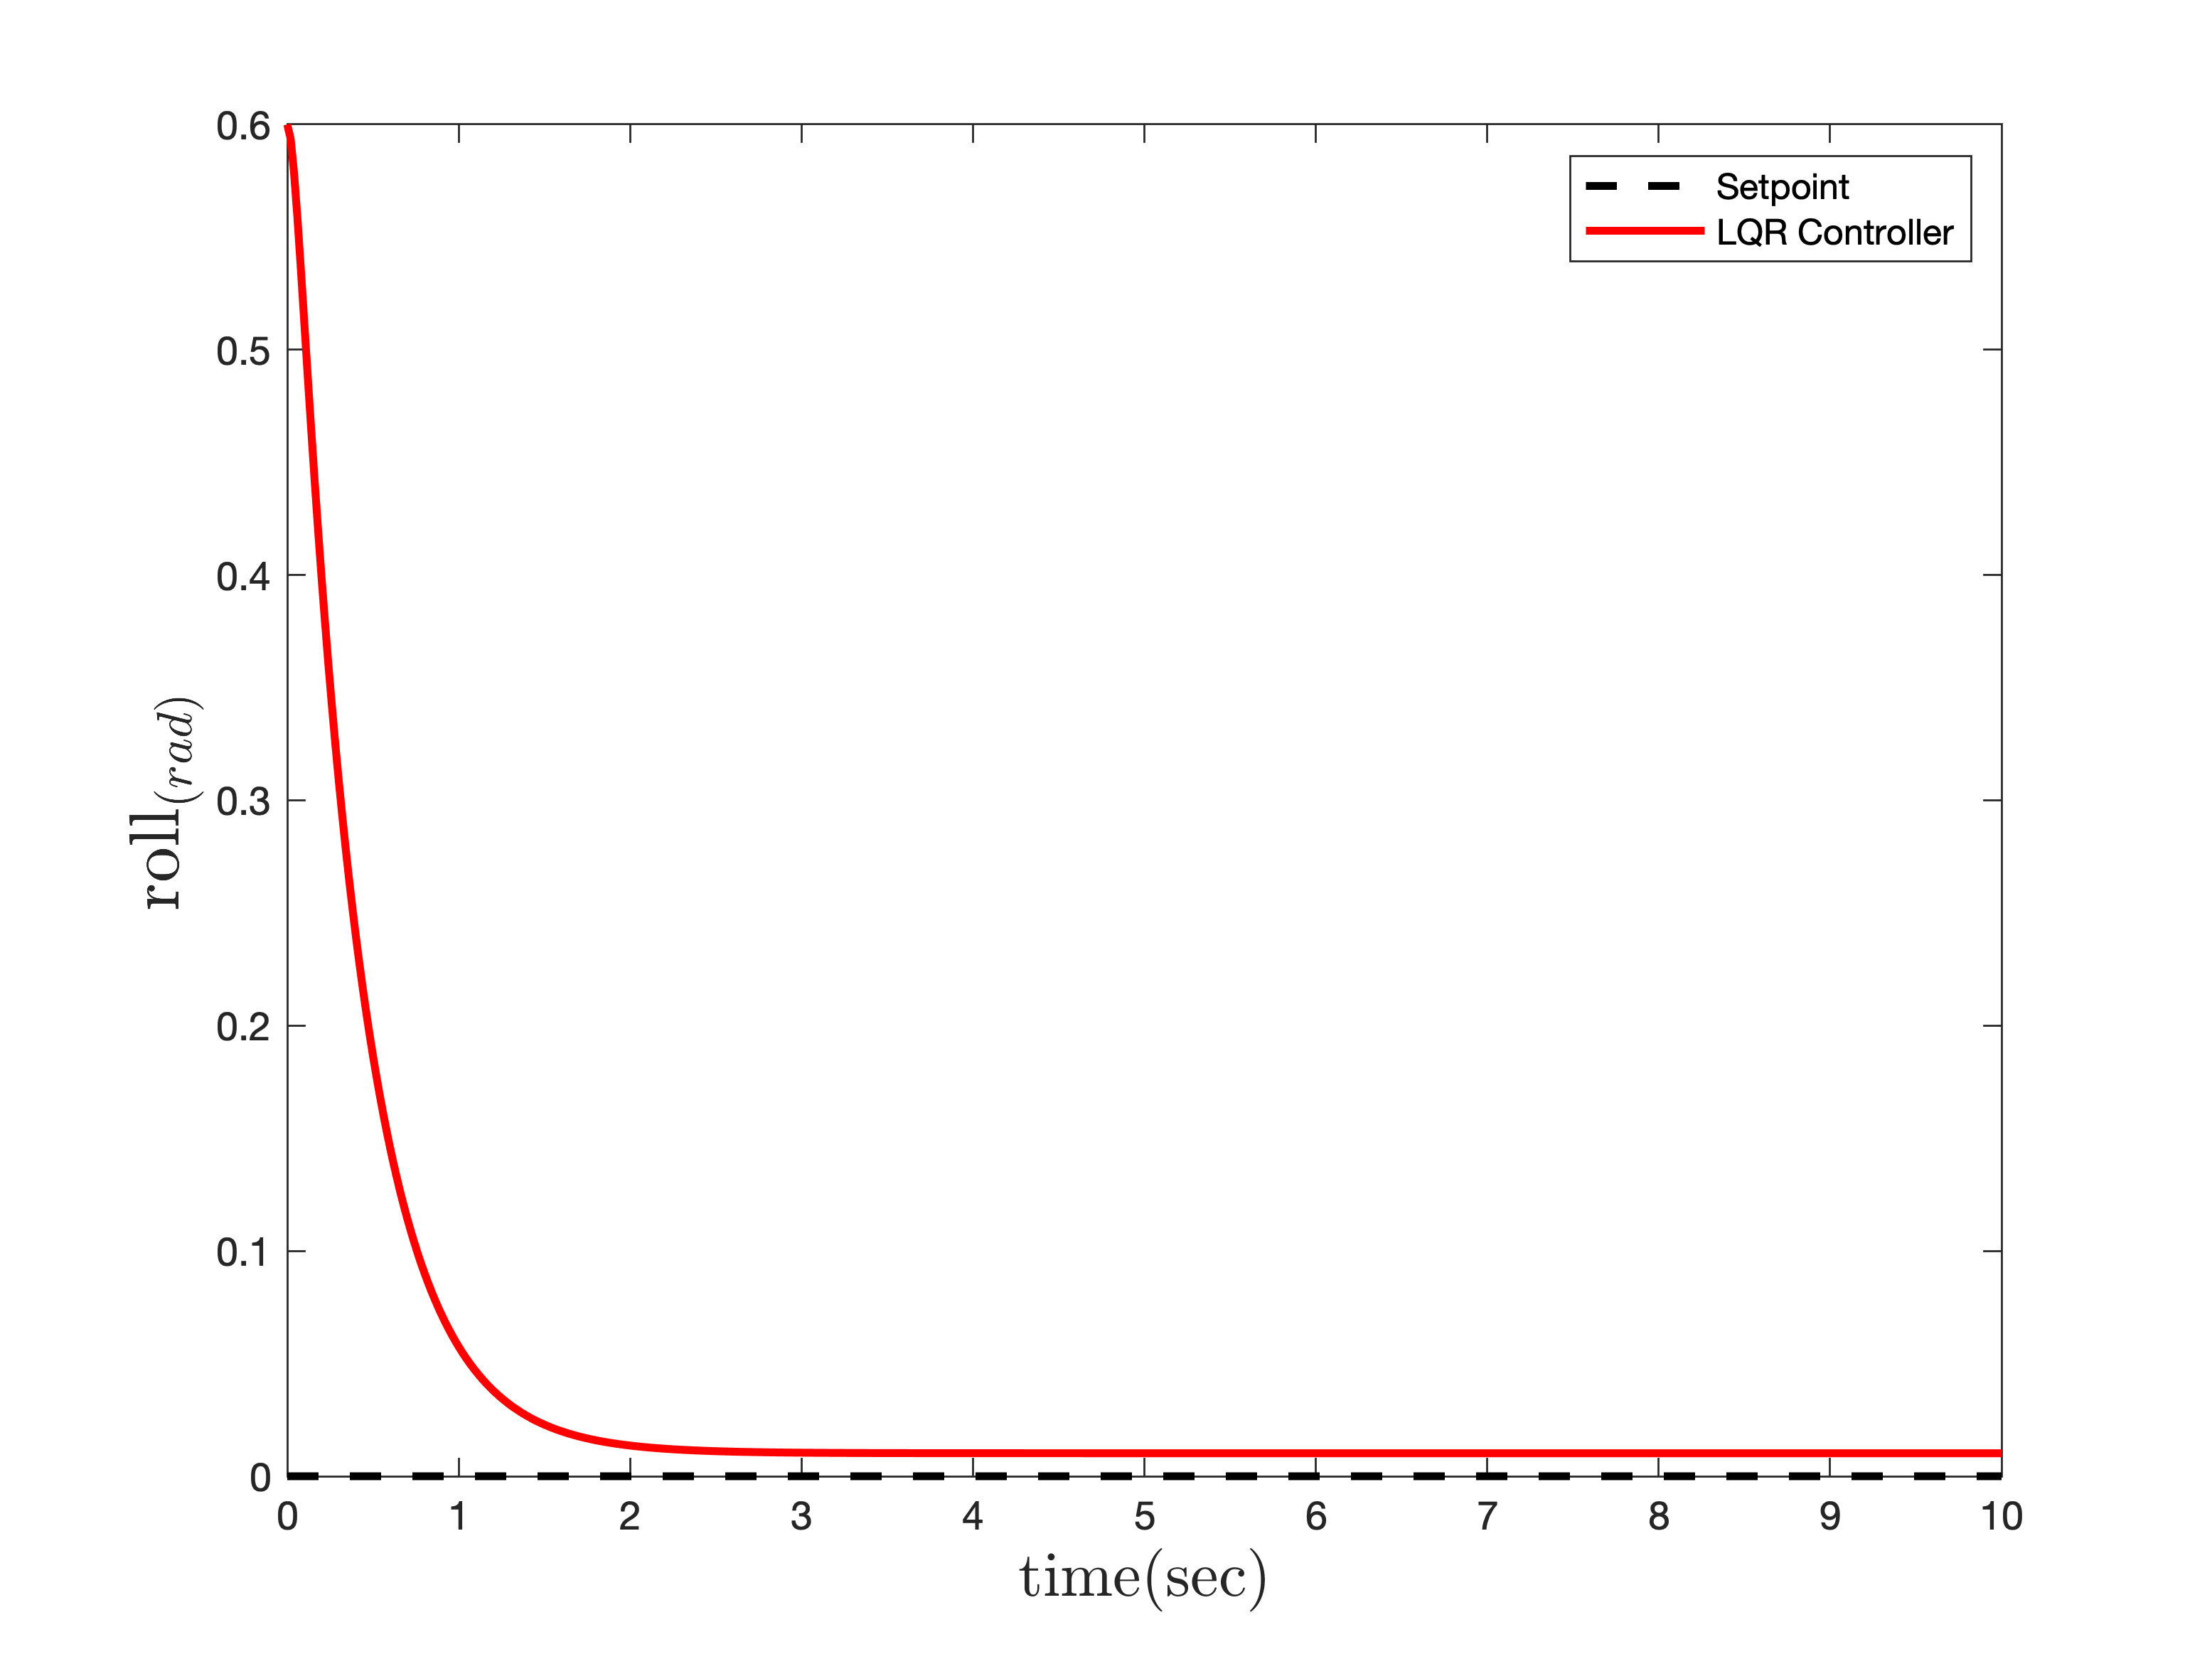
\includegraphics[width=.48\linewidth]{../Figures/MIL/LQR/Roll/lqr_roll_nn.png}
	\centering
	\caption{عملكرد کنترل‌کننده \lr{LQR} در کنترل زاويه رول (تعقیب ورودی صفر)}
	\label{lqr_roll_figure_simulation}
\end{figure}
\begin{figure}[H]
	\centering
	\subfigure[موتور شماره دو]{
		\centering
		\includegraphics[width=.45\linewidth]{../Figures/MIL/LQR/Roll/lqr_roll_Omega_2_nn.png}
	}
	\subfigure[موتور شماره چهار]{
		\centering
		\includegraphics[width=.45\linewidth]{../Figures/MIL/LQR/Roll/lqr_roll_Omega_4_nn.png}
	}
	\caption{‫‪فرمان کنترلی موتورهای دو و چهار در کنترل زاویه رول (تعقیب ورودی صفر)}
\end{figure}
\بدون‌تورفتگی همانطور که از شکل
\ref{lqr_roll_figure_simulation}
مشخص است، زمان نشست در حدود دو ثانیه است و خطای ماندگار وجود دارد.